\section{VQA and QNN}
\begin{itemize}
    \item Basic concepts: \textbf{Cost function, ansatz, gradients, optimizers}
    \item Global and local cost function
    \item Some illustration?
\end{itemize}

Hybrid techniques involving Quantum circuits and Classical optimizers have been proposed to overcome the restrictions of Noisy Intermediate-Scale Quantum (NISQ) \cite{brooksQuantumSupremacyHunt2019} devices. 
Those constraints are the absence of fault-tolerant design, the limitation of qubit number per processor, and executable circuit depth. 
Moreover, quantum gates are static by design, which means every new data input to a quantum algorithm will produce a different quantum circuit.

Quantum circuits with trainable parameters can be created using Variational Quantum Algorithms (VQAs) \cite{cerezo2021variational}, which act as reusable circuit templates for quantum computers.
On the other hand, the classical optimizer perceives variational circuits as a black box that yields outputs from inputs and the trainable parameter.

Consider a simple problem that we want to solve using VQA, given the access to the training data.
The first step is to define a \textit{cost function} $C$ to search for a solution, we aim to minimize this cost function during the training process.
Then, we develop an \textit{ansatz}, this is the unitary operation that depends on a set of parameters $\theta$. We aim to train this ansatz to optimize $\theta$ such that the cost function $C$ reaches it minimum, thus satisfy this equation:
\begin{equation}
    \theta^* = \underset{\theta}{\arg \min} C(\theta)
    \label{optimize theta with ansatz}
\end{equation}

In short, the cost function $C(\theta)$ is calculated using the Quantum computer, while the classical optimizers train the parameter $\theta$. Figure \ref{VQA diagram} elaborates the VQA architecture and process in more details.

\begin{figure}
    \centering
    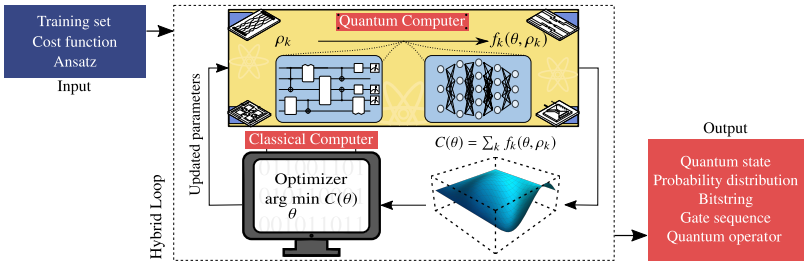
\includegraphics[width=\textwidth]{LiteratureReview/Appendices/vqadiagram.png}
    \caption{
    An illustrative diagram of VQA. The algorithm receives: 
    A cost function $C(\theta)$ for $\theta$ is a set of parameters that encodes the solution; 
    An ansatz that receive trainable parameter $\theta$ in the hybrid loop to solve the task;
    A set of training data $\{\rho_k\}$.
    For each iteration, we use the quantum computer to calculate the cost, then pass this information to the classical computer that use an optimizer to navigate the cost landscape $C(\theta)$ and solve the problem in Eq. (\ref{optimize theta with ansatz}).
    The output of VQA is an estimate of the solution to the problem, which can take forms as in the red box.
    Figure from ref \cite{cerezo2021variational}.
    }
    \label{VQA diagram}
\end{figure}

\subsection{The Cost function}
Encoding the problem into a cost function is the first step to solve a problem using VQA.
This is the same cost function compared to classical machine learning, it maps the values of the trainable parameters $\theta$ into real numbers.
For a function $f$ that receives input states $\{\rho_k\}$, observables $\{O_k\}$, and a parameterized circuit $U(\theta)$, the cost is expressed as:
\begin{equation}
    C(\theta) = f(\{\rho_k\}, \{O_k\}, U(\theta)) \;,
\end{equation}
or this form with a set of functions $\{ f_k \}$:
\begin{equation}
    C(\theta) = \sum_k f_k(\Tr[ O_k U(\theta) \rho_k U^\dagger(\theta) ]) \;,
    \label{Cost function}
\end{equation}

There are some criteria in construction of a cost function: 
(1) The cost function must be 'faithful' and 'operational meaningful', such that the minimum of $C(\theta)$ should correspond to the solution of the problem, and the lower cost function indicate a better solution in general;
(2) Cost function must be 'efficiently estimated' by measurement on quantum computer and classical post processing;
(3) The cost must be 'trainable', such that the parameters $\theta$ should be efficiently optimized.

\subsection{The Ansatzes}
\begin{figure} 
    \centerline{
        \Qcircuit @C=1em @R=0em {
        & \multigate{4}{U_1(\theta_1)}    & \multigate{4}{U_2(\theta_2)}    & \qw &        & & \multigate{4}{U_L(\theta_L)}   & \qw\\
        & \ghost{U_1(\theta_1)}           & \ghost{U_2(\theta_2)}           & \qw &        & & \ghost{U_L(\theta_L)}          & \qw\\
        & \ghost{U_1(\theta_1)}           & \ghost{U_2(\theta_2)}           & \qw & \cdots & & \ghost{U_L(\theta_L)}          & \qw\\
        & \ghost{U_1(\theta_1)}           & \ghost{U_2(\theta_2)}           & \qw &        & & \ghost{U_L(\theta_L)}          & \qw\\
        & \ghost{U_1(\theta_1)}           & \ghost{U_2(\theta_2)}           & \qw &        & & \ghost{U_L(\theta_L)}          & \qw\\
        \gategroup{1}{2}{5}{7}{.7em}{--}
        }
    }
    \centerline{$U(\theta)$}
    \caption{
        A diagram of an ansatz.
        The unitary $U(\theta)$ receives parameters $\theta$ is expressed by $L$ layers of unitaries $U_l(\theta_l)$ for $l$ is the layer indices.
    }\label{Ansatz diagram}
\end{figure}

The 'ansatze' is the parameterized circuit, parameterized unitary, or variational circuit.
In general, the parameters $\theta$ are determined by the form of the ansatz, and thus can be trained to minimize the cost.
The ansatz structure can be defined based on the problem (called 'problem-inspired ansatze'), or a generic structure (called 'problem agnostic') that can be used without any relevant information available.
The cost function in Eq. (\ref{Cost function}) encodes the parameters $\theta$ in an unitary $U(\theta)$ and apply to the input states of the circuit. The figure \ref{Ansatz diagram} shows that $U(\theta)$ can be expressed as a product of $L$ continuously unitaries:
\begin{equation}
    U(\theta) = U_L(\theta_L) \cdots U_2(\theta_2) U_1(\theta_1)\;,
\end{equation}


\subsection{The Gradients}
After defining the cost function and ansatz, we train the parameter $\theta$ to solve the problem in Eq. (\ref{optimize theta with ansatz}).
The cost function gradient helps the optimizer to find the global minima. 
Consider the cost function in Eq. (\ref{Cost function}), for a parameterized unitary $e^{i \theta_l \sigma}$, let $\theta_l$ be the $l$-th element of $\theta$, $\sigma_l$ is a Pauli operator. 
We can evaluate the gradient with the Parameter-shift rule:
\begin{equation}
    \frac{\partial C}{\partial\theta_l}
    = \sum_k \frac{1}{2 \sin{\alpha}} 
    \left( 
        \Tr[O_k U^\dagger(\theta_+) \rho_k U(\theta_+)] 
        - \Tr[O_k U^\dagger(\theta_-) \rho_k U(\theta_-)]
    \right) \;,
    \label{Parameter-shift rules}
\end{equation}
with $\theta_{\pm} = \theta \pm \alpha e_l$, $\alpha \in \mathbb{R}$ and $e_l$ is a vector such that its $l$-th position have the value of 1, or else 0.

Essentially, we can shift the $l$-th parameter by some amount $\alpha$ and the Eq. (\ref{Parameter-shift rules}) will evaluate the gradient. 


\subsection{The Optimizers}
The accuracy of VQA greatly depends on the optimization method.
Typically, we can achieve the solution by making successive moves along directions indicated by the gradient.
This approach of optimization is within the scope of Stochastic Gradient Descent (GSD).
One example of GSD is the ADAM optimizer \cite{kingmaAdamMethodStochastic2014}

\subsection{About QNN}
\almarginpar{I thought the VQA and QNN reviews would be more extensive?}VQA is also the most widely used method for developing Quantum Neural Network (QNN) circuits. 
As a result, QNN inevitably inherited some of VQA's flaws.
Many Quantum Machine Learning models suffer from the unsolvability Barren Plateaus \cite{zhaoReviewQuantumNeural2021} that prevent the growth of circuit depth and lead the trainable parameters to a dead end.
When training a QNN framework with a large number of qubits, this phenomenon occurs; the objective function becomes flat, making it nearly impossible to estimate the gradient, \cite{mccleanBarrenPlateausQuantum2018, zhaoAnalyzingBarrenPlateau2021} causing inefficiency in circuit training. 

